% LTL paper, v4 = merge of two independent hostile reviews (2026-07-10).
% Review A (second Fable instance): frontier hash-fold framework (the
% lemma did not cover its own uses as written), dangling R4/R5 labels,
% deny-only label semantics, Table 1 caption, r_1 as raw bytes, exact
% RFC 9162 figure. Review B (GPT-5.6): G2/abstract narrowed to what
% Prop 1 proves, residual-trust sentence at honest width, freshness and
% self-reference disclaimers, softened novelty/mechanization claims,
% head-encoding documented, claim-matrix table. Both reviews' findings
% independently re-verified before adoption.
\documentclass[11pt]{article}
\usepackage[a4paper,margin=1.1in]{geometry}
\usepackage{amsmath,amssymb,amsthm}
\usepackage{xcolor}
\usepackage[colorlinks=true,linkcolor=blue!60!black,citecolor=blue!60!black,urlcolor=blue!60!black]{hyperref}
\usepackage{enumitem}
\usepackage{booktabs}
\usepackage{lmodern}
\usepackage{microtype}
% this TeX install's format ships righthyphenmin=1 ('it-s'); restore standard
\lefthyphenmin=2 \righthyphenmin=3
\usepackage{tikz}
\usetikzlibrary{fit,positioning,decorations.pathreplacing}

\newtheorem{theorem}{Theorem}
\newtheorem{lemma}{Lemma}
\newtheorem{proposition}{Proposition}
\newtheorem{corollary}{Corollary}
\newtheorem{definition}{Definition}
\theoremstyle{remark}
\newtheorem{remark}{Remark}

\newcommand{\authortodo}[1]{\textcolor{red}{\textbf{[AUTHOR TODO: #1]}}}
\newcommand{\hash}{\mathsf{H}}
\newcommand{\hleaf}{\mathsf{h}_{\mathsf{leaf}}}
\newcommand{\hnode}{\mathsf{h}_{\mathsf{node}}}
\newcommand{\MTH}{\mathsf{MTH}}
\newcommand{\Root}{\mathsf{Root}}
\newcommand{\ConsRec}{\mathsf{ConsRec}}
\newcommand{\Path}{\mathsf{Path}}
\newcommand{\obs}{\mathsf{obs}}
\newcommand{\allowed}{\mathsf{allowed}}
\newcommand{\clean}{\mathsf{clean}}
\newcommand{\accept}{\mathsf{accept}}
\newcommand{\Fp}{\mathbb{F}_{2^{255}-19}}

\title{The Lean Transparency Log:\\ Distributing Kernel-Checked Correctness Evidence\\ for Deployed Ed25519 Implementations}
\author{Olaf Horvath\\
\small Olaf.Horvath@zkdefi.org \quad ORCID 0009-0004-8008-5805
% \authortodo{if you have any institutional or personal-domain affiliation,
% use it here instead of / alongside the zkdefi.org address}
}
\date{July 2026 (revised)}

\begin{document}
\maketitle

\begin{abstract}
Interactive theorem provers can certify functional correctness of deployed
cryptographic code, but the resulting assurance is expensive to consume:
re-checking a realistic proof corpus requires a proof toolchain and hours of
kernel time, which excludes almost every downstream user. We describe the
Lean Transparency Log (LTL), an RFC~9162-style transparency log whose leaves
are \emph{replay attestations}: signed statements that the Lean~4 proofs of a
specific Rust repository, at a specific git commit, re-check with exactly
their documented axiom sets. Consumers verify one signature and a logarithmic
inclusion proof in milliseconds; the kernel time is paid once, by the log
operator.

This paper makes the trust model precise and proves the consumer-facing
security claims. We define the attestation-transparency setting, give an
explicit adversary model in which the operator may be malicious, and prove:
completeness and soundness of the inclusion verifier (soundness via an
explicit reduction extracting a SHA-256 collision), the analogous consistency
statement, safety of the consumer's head-pinning state machine (same-size
equivocation yields transferable evidence, and local pinning rejects
inconsistent extensions), and \emph{verdict
integrity}---consumers re-derive verification verdicts locally from observed
axiom cones, so the operator is trusted only for \emph{observations}, never
for \emph{verdicts}. A further design choice ties the log to its own subject
matter: tree heads are signed by a binary built from the very Ed25519
implementation whose correctness certificates are leaves of the log. We
report a small production deployment covering four verified production
Ed25519 implementations, state exactly what the accumulated evidence does and
does not establish, and outline the mechanization of this paper's theorems in
Lean as the natural next step.
\end{abstract}

\section{Introduction}\label{sec:intro}

Formal verification of deployed cryptographic code has matured from research
prototypes to substantial artifacts: verified-by-construction libraries such
as HACL*~\cite{hacl} and Fiat-Crypto~\cite{fiatcrypto} ship in mainstream
software, and post-hoc verification pipelines such as Aeneas~\cite{aeneas}
make it possible to state and prove theorems about existing production Rust
code. The corpus underlying this paper is of the latter kind: four production
Ed25519 implementations---upstream \texttt{curve25519-dalek}/%
\texttt{ed25519-dalek} (one implementation: the curve crate and the
signature crate atop it) and three deployed forks (Solana, RISC~Zero,
Betrusted)---each carry Lean~4~\cite{lean4} certificates, proven against that
fork's own extracted model, covering field arithmetic over $\Fp$, the
complete twisted Edwards laws~\cite{edwards,twisted}, scalar arithmetic
mod~$\ell$, encoding/decoding with constructive point decompression, and a
four-tier characterization of signature verification~\cite{eddsa,rfc8032}
whose strongest tier states: the extracted verifier accepts iff the
signature's $R$ component decompresses to a valid curve point equal to
$[k](-A) + [s]B$. Section~\ref{sec:corpus} states these theorems precisely.

The economics of \emph{consuming} such evidence are poor: re-checking one
fork's certificates takes ${\approx}30$ minutes of Lean kernel time and a
pinned toolchain. A wallet, a package manager, or an autonomous agent
choosing a cryptographic backend cannot pay this per decision---and need not:
a deterministic re-check yields a fact that can be attested once and
distributed. This is the classic transparency-log trade---Certificate
Transparency~\cite{ct1,ct2} for certificate issuance, Sigstore's
Rekor~\cite{sigstore} for signing events and supply-chain
attestations~\cite{intoto}, key transparency~\cite{coniks}, checksum
databases---applied to a payload with different trust semantics: evidence of
machine-checked mathematical truth, together with its exact assumption set.

\paragraph{Contributions.} The hash structure and proof algorithms are
RFC~9162 verbatim, and we claim no novelty for any individual component. The
contributions are:
\begin{enumerate}[itemsep=1pt]
\item \textbf{A precise trust model for attestation transparency over
  machine-checked proofs} (\S\ref{sec:model}), in which the log operator is
  trusted for \emph{observations} (``this is what the kernel printed'') but
  never for \emph{verdicts} (``these proofs are acceptable''), because
  consumers re-derive every verdict locally from the observed axiom cones
  carried in each attestation.
\item \textbf{Security proofs for the consumer-facing claims}
  (\S\ref{sec:security}): completeness and soundness of the RFC~9162
  inclusion verifier as used here (soundness as an explicit extractor that
  turns any accepting proof for a non-member leaf into a SHA-256 collision),
  the analogous consistency statement, safety of the consumer's pin-store
  state machine, and verdict integrity. The statements are elementary but,
  written out, they pin down exactly which assumption carries which claim.
\item \textbf{Boundary-exact axiom auditing} (\S\ref{sec:construction}):
  observed axiom cones are matched against per-theorem documented boundaries
  \emph{exactly, in both directions}---an unexpected axiom and a missing
  boundary axiom are both flagged.
\item \textbf{A self-referential (not circular) signing design and a deployed
  instance} (\S\ref{sec:selfref}, \S\ref{sec:deployment}): tree heads are
  signed by a binary built from the pinned source of exactly the Ed25519
  implementation attested in the log, with the operator's own Merkle
  self-check of that leaf published alongside every signed head; and a small,
  reproducible production deployment over the four-fork corpus, including a
  measurement of proof portability across real forks.
\end{enumerate}

\paragraph{Non-claims.} The LTL does not mechanize cryptographic security
proofs---that bridge is being built by EasyCrypt and its
relatives~\cite{easycrypt}. It does not establish correctness of any binary,
of SHA-512, of wire-format parsers, of the signing path, or any side-channel
property; \S\ref{sec:deployment} enumerates the assumption set in full. It
bridges an adjacent, mostly empty gap: type-theory-certified artifacts
lack distribution infrastructure, and we are unaware of a deployed
transparency log designed to carry kernel-replay attestations together
with theorem-level assumption boundaries.\footnote{The
acronym LTL collides with linear temporal logic~\cite{pnueli}; the collision
is acknowledged.}

\section{Background: the proof corpus}\label{sec:corpus}

The corpus is a stack of theorems about extracted code, each stated through
a denotation from machine representation to mathematics. Field elements are
five 51-bit limbs denoting
$[\![(a_0,\dots,a_4)]\!] = \sum_i a_i 2^{51i} \bmod p$ with
$p = 2^{255}-19$, and every operation carries a two-clause
specification---the value is right \emph{and} the representation invariant
is preserved, e.g.
\[
\forall a\, b.\;\; \mathsf{bnd}\,a \Rightarrow \mathsf{bnd}\,b \Rightarrow
\exists c.\;\; \mathsf{mul}\,a\,b = \mathsf{ok}\,c \,\wedge\,
\mathsf{bnd}\,c \,\wedge\, [\![c]\!] = [\![a]\!]\cdot[\![b]\!].
\]
Point operations are proven to implement the complete twisted Edwards
addition law on $E : -x^2+y^2 = 1+d\,x^2y^2$ over $\Fp$,
\[
(x_1,y_1)+(x_2,y_2) \;=\;
\left(\frac{x_1y_2+x_2y_1}{1+d\,x_1x_2y_1y_2},\;
      \frac{y_1y_2+x_1x_2}{1-d\,x_1x_2y_1y_2}\right),
\]
including the completeness fact that makes it branch-free ($a=-1$ is a
square and $d$ a non-square in $\Fp$, so the denominators never
vanish~\cite{edwards}).

\paragraph{The signature apex as a lifting ladder.} The signature-tier
result is not one theorem but a ladder of four, each lifting the previous
one to a stronger domain; the payload the log distributes is the
\emph{conjunction} of the four, and their separation is what makes the
residual hypotheses legible. Write $\accept(A,m,R,s)$ for ``the extracted
verifier returns \textsf{ok}'', let $k$ be the scalar produced by the hash
oracle $H(R,A,m)$ with \emph{no properties assumed of $H$}, and let $r_1$
be the 32-byte $R$ component exactly as it appears in the signature (raw
bytes; no canonicity of them is presupposed). Each
tier is proven for the extracted code under the wire-format
hypotheses~$\mathcal{W}$ (the signature parses to an internal
representation and the relevant compressed points re-encode; these
outcomes are assumed, not proven---their byte-level specifications are
part of the open frontier recorded in \S\ref{sec:limitations}).
\begin{description}[itemsep=3pt,leftmargin=1.6em]
\item[T1 (byte apex).] $\accept(A,m,R,s) \Leftrightarrow
  \mathsf{compress}([s]B-[k]A) = r_1$. Acceptance is byte-equality of the
  verifier's recomputed encoding with the signature's $R$ bytes---a
  statement purely about the extracted control flow.
\item[T2 (canonical half-lift).] The recomputed bytes
  $\mathsf{compress}([s]B-[k]A)$ \emph{are} the canonical encoding of the
  group element $[k](-A)+[s]B$; that is, $\mathsf{compress}$ agrees on this
  input with the mathematical canonical-encoding function. T1 and T2 give
  $\accept \Leftrightarrow \mathsf{enc}([k](-A)+[s]B) = r_1$.
\item[T3 (injectivity / point equation).] Canonical encodings are
  injective on $E(\Fp)$: if a valid curve point $P$ has $\mathsf{enc}(P) =
  r_1$ then $P = [k](-A)+[s]B$. Injectivity is exactly where
  non-squareness of $d$ re-enters---it keeps $1 + d y^2 \neq 0$, so the
  curve equation determines $x^2$ from $y$ and the encoding is one-to-one.
\item[T4 (constructive full lift).] $\accept(A,m,R,s) \Leftrightarrow
  \mathsf{decompress}(R) = [k](-A)+[s]B$, with the extracted
  $\mathsf{decompress}$ proven to realize the mathematical inverse of
  $\mathsf{enc}$: exact byte parsing, the $(p+3)/8$-power square root, and
  sign-bit root selection (for $x \neq 0$ the two roots $x$ and $p-x$
  differ in parity since $p$ is odd, so the stored sign bit selects
  correctly; at $x = 0$ the roots coincide and a set sign bit is rejected,
  per RFC~8032---the theorem, an \emph{iff} over the extracted code,
  covers this branch by construction).
\end{description}
The lift is monotone in strength---T1 is about bytes the code emits, T4 is
about the group element a third party would recover from $R$---and each
step names precisely one new mathematical fact (canonicity, injectivity,
constructive inversion). A consumer that only trusts byte equality can
stop at T1; a consumer reasoning about the underlying group element relies
on T4. Both are in the corpus, separately certified, and the log carries
all four so the consumer chooses the tier, not the operator.

\paragraph{Axiom cones.} Each theorem's \emph{axiom cone}---the set of
axioms its proof ultimately depends on, as reported by Lean's
\texttt{\#print axioms}---is pinned exactly: the standard three axioms for
the foundational certificates, plus an enumerated oracle boundary
(SHA-512 and the wire-format types) at the four apex tiers. It is this
exact set, not a pass/fail label, that each leaf carries and each consumer
re-checks (\S\ref{sec:auditing}). Appendix~\ref{app:tiers} restates the
ladder with the Lean theorem names; Appendix~\ref{app:axioms} lists the
per-fork allowed sets verbatim.

\section{Related work}\label{sec:related}

Certificate Transparency~\cite{ct1,ct2} supplies the data structure and
proof algorithms, used here unchanged; the underlying history-tree technique
originates with Crosby and Wallach~\cite{crosby}. Dowling, G\"unther, Herath
and Stebila~\cite{dghs} give formal security definitions and proofs for the
CT primitives (logging schemes, inclusion, consistency); the analysis in
\S\ref{sec:security} is in the same spirit, specialized to this system's
verifier and stated so that each claim can later be mechanized in Lean
(\S\ref{sec:next}). Rekor within Sigstore~\cite{sigstore} is the closest
deployed system: a transparency log over signing events and supply-chain
attestations such as in-toto~\cite{intoto} link metadata; its payloads attest
\emph{process} (who signed, how an artifact was built), whereas LTL leaves
attest kernel-checked mathematical statements together with their assumption
sets, and the consumer re-derives verdicts rather than trusting labels. Key
transparency~\cite{coniks} and checksum databases share the pattern with
different payloads. Proof-carrying code~\cite{pcc} ships proofs to consumers
who check them; the LTL serves consumers who cannot run any checker,
replacing proof transport with attestation, inclusion, and signature---at
the cost of trusting the operator's kernel run, a cost the design minimizes
(\S\ref{sec:model}) but does not eliminate. Cheval, Moreira and Ryan
formally verify transparency protocols themselves~\cite{cheval}; our
direction is the complement (we log the verification), and \S\ref{sec:next}
proposes meeting in the middle. Verified Merkle tree implementations exist,
notably in EverCrypt~\cite{evercrypt}; \S\ref{sec:next} builds on that
precedent rather than claiming it.

\section{System and trust model}\label{sec:model}

\subsection{Roles and scheme syntax}

The system has exactly two roles with deliberately asymmetric costs and
capabilities. The \emph{operator} (one per log) owns a Lean toolchain,
replays proof corpora, holds the log's signing key, and bears append-only
obligations. \emph{Consumers} (unbounded in number) hold the operator's
public key, receive small evidence files, and verify: the Merkle
inclusion core is roughly 25 lines of standard-library code
(Appendix~\ref{app:verifier}); the full standalone consumer---head
signature, consistency, mirror audit---is ${\approx}150$ lines
(\S\ref{sec:pinstore}), atop an Ed25519 backend. Nothing a consumer
does requires a theorem prover.

We phrase the system as an \emph{attestation-transparency scheme}, in the
style of the logging schemes of Dowling et al.~\cite{dghs}, so that the
security goals below can name its algorithms precisely.

\begin{definition}[Attestation-transparency scheme]\label{def:scheme}
A scheme $\Pi$ is a tuple of algorithms over a hash function $\hash$ and a
signature scheme $\mathsf{Sig}$:
\begin{itemize}[itemsep=1pt,leftmargin=1.4em]
\item $\mathsf{KeyGen} \to (sk, pk)$: the operator's head-signing keypair.
\item $\mathsf{Append}(sk, \mathbf{D}, a) \to (\mathbf{D}', \sigma)$:
  appends attestation-leaf $a$ to the ordered leaf list $\mathbf{D}$,
  returning the new list and a signed tree head
  $\sigma = \mathsf{Sig}.\mathsf{Sign}(sk, (|\mathbf{D}'|, \MTH(\mathbf{D}'), t))$.
\item $\mathsf{ProveIncl}(\mathbf{D}, m) \to P$ and
  $\mathsf{VerifyIncl}(pk, d, m, \sigma, P) \to \{0,1\}$: the membership
  proof and its verifier (\S\ref{sec:tree}, Appendix~\ref{app:verifier}).
\item $\mathsf{ProveCons}(\mathbf{D}, n_0) \to C$ and
  $\mathsf{VerifyCons}(pk, \sigma_0, \sigma_1, C) \to \{0,1\}$: the
  append-only (consistency) proof between two signed heads and its verifier
  (\S\ref{sec:tree}).
\item $\mathsf{Verdict}(\allowed, a) \to \{\clean, \neg\clean,
  \bot\}^{|a|}$: the consumer's per-certificate verdict function
  (\S\ref{sec:auditing}), parameterized by the consumer's \emph{own}
  allowed-axiom table $\allowed$ and taking \emph{no} operator label as
  input.
\end{itemize}
$\MTH$, $\mathsf{ProveIncl/VerifyIncl}$ and $\mathsf{ProveCons/VerifyCons}$
are the RFC~9162 algorithms, defined in \S\ref{sec:tree}; $\mathsf{Append}$
and $\mathsf{Verdict}$ are specific to this system.
\end{definition}

\subsection{Adversary model}

We consider a probabilistic polynomial-time adversary $\mathcal{A}$ that
controls the network (may reorder, replay, drop, or forge messages to
consumers) and may \emph{be} the operator. A malicious operator may sign
arbitrary tree heads, construct arbitrary leaves, present different views to
different consumers, and label attestations arbitrarily. The single
capability we do \emph{not} model cryptographically is falsification of
kernel observations: an operator who reports an axiom cone that the Lean
kernel never printed is lying about a physical event on its own machine, and
no log structure can exclude this; \S\ref{sec:model:residual} isolates this
residual trust precisely. Standard assumptions: SHA-256 is collision
resistant; Ed25519 (as instantiated by the signing binary) is EUF-CMA
secure; the consumer obtained the operator's true public key (trust on first
use; \S\ref{sec:limitations}).

\subsection{Security goals}\label{sec:model:goals}

These goals are what per-item signatures alone cannot supply: a set of
individually signed attestations cannot evidence a silent deletion
(nothing commits to completeness), cannot expose two-faced service
(independently valid views are incomparable), and offers no single value
a consumer can pin and demand extensions of. The Merkle tree is chosen
for these dishonesty-evidence properties, not for proof-size scaling,
which at this deployment's size is immaterial.

\begin{description}[itemsep=2pt]
\item[G1 (Membership).] If a consumer accepts a receipt for attestation $a$
  against a signed head, then $a$ is a leaf of the tree committed by that
  head---any other outcome exhibits a SHA-256 collision or an Ed25519
  forgery. (Theorem~\ref{thm:sound}, Proposition~\ref{prop:pin}.)
\item[G2 (Append-only with fork evidence).] A consumer's accepted view of
  the log only ever grows by extension, and two accepted heads of
  \emph{equal} tree size with different roots are, together, transferable
  publicly verifiable evidence of equivocation. Unequal-size split views
  are not exposed by the head pair alone; they are exposed by the public
  leaf mirror (\S\ref{sec:pinstore}), from which any party recomputes
  every prefix root (itself operator-published, hence witness-dependent;
  \S\ref{sec:limitations}), or by an external witness.
  (Theorem~\ref{thm:consistency}, Proposition~\ref{prop:pin}.)
\item[G3 (Verdict integrity).] The verdict a consumer derives for a
  certificate depends only on the observed axiom cone in the leaf and the
  consumer's \emph{own} copy of the allowed axiom sets; the operator's
  pass/fail labels can deny (a certificate the operator does not itself
  mark proven never counts) but can never grant.
  (Proposition~\ref{prop:verdict}.)
\end{description}

\subsection{The residual trust, isolated}\label{sec:model:residual}

Goals G1--G3 reduce the operator's trusted role to a single sentence,
which we state at its honest width: \emph{``the operator executed the
declared replay procedure against the exact pinned source and dependency
state, using the declared toolchain, and bound the resulting kernel
outputs faithfully to the correct theorem entries of the attestation.''}
Checkout, dependency state, theorem-to-entry binding, and output parsing
are all inside this observation pipeline---the first deployed run failed
on precisely such a defect (\S\ref{sec:deployment}). Everything
else---membership, history, verdicts---is either cryptographically
enforced or locally re-derived. An
operator that labels a dirty cone ``clean'' gains nothing (G3); an
attestation that omits observed cones is treated as unverifiable; an
operator that rewrites history is caught with transferable evidence (G2).
An operator that fabricates observations can only be caught by independent
replay, which any party with a Lean toolchain can perform from the pinned
commit---the design makes such an audit cheap to \emph{target} (the claim
is exact: repository, commit, toolchain, expected cones) even though it is
expensive to \emph{run}.

\subsection{Verdicts are the consumer's, not the operator's}\label{sec:model:card}

The design choice behind G3 is what most distinguishes this system from
prior attestation transparency, so we state it as a principle rather than
a mechanism. In systems like Rekor~\cite{sigstore} a consumer learns
\emph{that} something was attested and trusts the issuer's assessment of
it; the payload's meaning is the issuer's to declare. Here the payload is
a set of \emph{observations}---the literal \texttt{\#print axioms} output
per theorem---and the assessment ($\clean$ or not) is computed by
$\mathsf{Verdict}$ (Definition~\ref{def:scheme}) from those observations
against the consumer's own table $\allowed$. Concretely:
\begin{itemize}[itemsep=1pt,leftmargin=1.4em]
\item The allowed set $\allowed(c)$ is not shipped by the operator at
  verification time; it is part of the consumer's tooling, small enough to
  audit by hand (Appendix~\ref{app:axioms}: 7--11 axiom names per fork),
  and re-derivable \emph{up to naming} from the theorem statements---%
  Lean's foundational three, plus, for the apex tiers, placeholders for
  exactly those primitives the theorem deliberately leaves opaque (the
  hash, the wire format); the placeholder \emph{names} themselves are
  fixed by the fork's extracted surface and read off from
  Appendix~\ref{app:axioms}.
\item That an independently written $\allowed$ meets the deployed
  observations \emph{exactly} is engineered, not coincidental: the corpus
  is minimized so that every axiom in a cone earns its place, and any
  reasonable reconstruction of ``what a correct proof of this statement
  must assume,'' once the fork's extraction naming is fixed, lands on the
  same finite set. When the consumer's requirement meets the supply
  exactly, verification is a set equality.
\item When it does not---a consumer who additionally requires SHA-512
  itself proven, say---the gap is exact and itemized (the boundary axioms
  of Appendix~\ref{app:axioms}), and the consumer's options are honest:
  accept a \emph{named} residual, decline, or discharge the missing
  boundary and let the resulting certificate enter the log. The log is
  additive in the same way requirements are; a stricter table is a roadmap,
  not a rejection.
\end{itemize}
The operator, in this picture, is not a judge whose verdict one trusts but
a witness whose \emph{observations} one re-adjudicates. G3
(\S\ref{sec:model:goals}, Proposition~\ref{prop:verdict}) is the formal
statement that this re-adjudication takes no positive input from the
operator's opinion: labels act, if at all, only as a conservative veto.

\section{The log construction}\label{sec:construction}

\subsection{Leaves: replay attestations}\label{sec:leaves}

A leaf is the canonical JSON serialization of an attestation recording: the
subject repository URL and git commit (which pins the entire source
tree through git's object identifiers---hardened SHA-1, noted here
because it is a weaker primitive than the log's own SHA-256); the
toolchain versions; the resource-control regime
under which the replay ran; and, per certificate, its name, replay status,
and the \emph{observed axiom cone}---the exact output of Lean's
\texttt{\#print axioms} for that theorem. For the corpus of
\S\ref{sec:corpus} each attestation carries 16 certificates.
Appendix~\ref{app:leaf} gives the leaf schema.

\subsection{Boundary-exact auditing}\label{sec:auditing}

Every certificate $c$ has a documented allowed axiom set $\allowed(c)$.
Foundational certificates must carry exactly Lean's three standard axioms
(\texttt{propext}, \texttt{Classical.choice}, \texttt{Quot.sound}); the four
signature-tier certificates additionally carry a per-fork, explicitly
enumerated boundary (an opaque SHA-512 oracle and opaque wire-format
types---e.g., eleven axioms in total for the upstream fork). Writing
$\obs(c)$ for the observed cone recorded in the leaf, define
\[
\clean(c) \;:\Longleftrightarrow\; \obs(c) = \allowed(c)
\quad\text{(equality of finite sets).}
\]
Deviation in \emph{either} direction---an unexpected axiom, or a missing
boundary axiom---falsifies $\clean$. The second direction matters for
these \emph{oracle} boundaries: a missing boundary axiom signals that the
theorem no longer consumes a primitive it deliberately left opaque. The
verifier does not attempt to distinguish the readings of that drift (a
genuinely strengthened proof; a changed theorem; a hash oracle discharged
by a placeholder rather than kept opaque; stale policy): it refuses to
classify, and rejects. Each
source repository enforces the same discipline in its own check scripts; the
log mirrors those sets, and consumers carry their own copies.

\subsection{Tree, heads, receipts}\label{sec:tree}

Let $\hash$ be SHA-256. Define, for a byte string $d$ and 256-bit values
$x,y$:
\[
\hleaf(d) = \hash(\texttt{0x00} \,\|\, d), \qquad
\hnode(x,y) = \hash(\texttt{0x01} \,\|\, x \,\|\, y).
\]
For a leaf list $D = [d_0,\dots,d_{n-1}]$ the RFC~9162 tree head is
\[
\begin{aligned}
\MTH([\,]) &= \hash(\varepsilon), \qquad
\MTH([d]) = \hleaf(d),\\
\MTH(D) &= \hnode\bigl(\MTH(D[0{:}k]),\, \MTH(D[k{:}n])\bigr),
\end{aligned}
\]
where $k$ is the largest power of two strictly less than $n$. The
\emph{inclusion path} for index $m$ is
\[
\Path(m, [d]) = [\,], \qquad
\Path(m, D) =
\begin{cases}
\Path(m, D[0{:}k]) \,\|\, [\MTH(D[k{:}n])] & m < k,\\
\Path(m-k, D[k{:}n]) \,\|\, [\MTH(D[0{:}k])] & m \ge k,
\end{cases}
\]
and the consumer's root-reconstruction function $\Root(v, m, n, P)$ is the
evident dual (Appendix~\ref{app:verifier}): fold the path back up, choosing
left/right by comparing $m$ with $k$ at each level.

\paragraph{Consistency.} A consistency proof $C$ lets a consumer check
that a size-$n_1$ tree \emph{extends} a size-$n_0$ tree it already pinned,
$0 < n_0 \le n_1$. We give the verifier as a function $\ConsRec$ that
reconstructs \emph{both} committed roots from $C$; it is the recursive
counterpart of RFC~9162~\S2.1.4, and we use this form (rather than the
RFC's iterative one) because the proofs of \S\ref{sec:security} induct on
it. On a proof $C$ interpreted as a list of nodes, with a flag $b$
recording whether the size-$n_0$ subtree's root is carried implicitly (the
pinned root) or explicitly in $C$:
\[
\ConsRec(n_0, n, C, b, r) =
\begin{cases}
(r, r) & n_0 = n,\ b,\ C = [\,],\\
(s, s) & n_0 = n,\ \neg b,\ C = [s],\\
\bigl(x,\, \hnode(y, s)\bigr) & n_0 \le k,\ C = C' \| [s],\\
\bigl(\hnode(s, x'),\, \hnode(s, y')\bigr) & n_0 > k,\ C = C' \| [s],
\end{cases}
\]
where $k$ is the largest power of two below $n$, $(x,y) =
\ConsRec(n_0, k, C', b, r)$ in the third case, and $(x',y') =
\ConsRec(n_0 - k, n - k, C', \bot, r)$ in the fourth (any shape mismatch
rejects). The consumer accepts $C$ between signed heads $(n_0, r_0)$ and
$(n_1, r_1)$ iff $n_0 = 0$, or $\ConsRec(n_0, n_1, C, \top, r_0) =
(r_0, r_1)$. We verified that this recursive form agrees with the deployed
iterative RFC~9162 verifier by \emph{exhaustive} differential testing over
every pinned/current size pair $1 \le n_0 \le n_1 \le 256$, each with the
honest proof and four adversarial mutations (wrong old root, wrong new
root, truncated and padded proofs): $164{,}224$ verifier invocations,
full agreement. The inclusion verifier of Appendix~\ref{app:verifier} was
checked the same way ($164{,}479$ invocations over all $m < n \le 256$).

The operator signs tree heads $(n, \MTH(D), t)$ with Ed25519; a
\emph{receipt} for a leaf is its index, its sibling path, and a signed
head. The signed payload is not the bare triple but the canonical JSON
serialization (sorted keys, fixed separators, UTF-8---injective on the
field set) of the head record, which additionally carries a protocol
version tag (\texttt{pacta.transparency.signed\_tree\_head.v1}) and the
log identity;
a head signature therefore transfers neither across logs nor across
protocol versions.

\subsection{The consumer pin store}\label{sec:pinstore}

Each consumer maintains a local pin $(n_{\mathrm{pin}}, r_{\mathrm{pin}})$,
updated by the following state machine on receiving a validly signed head
$(n', r')$:
\begin{itemize}[itemsep=1pt]
\item $n' = n_{\mathrm{pin}}$: accept iff $r' = r_{\mathrm{pin}}$; a
  mismatch is reported as \emph{equivocation}, the pair of signed heads is
  retained as evidence, and the state is poisoned (unrecoverable).
\item $n' > n_{\mathrm{pin}}$: accept iff a consistency proof from
  $(n_{\mathrm{pin}}, r_{\mathrm{pin}})$ to $(n', r')$ verifies; then update
  the pin.
\item $n' < n_{\mathrm{pin}}$: reject (rollback).
\end{itemize}
A freshness policy bounds head age; freshness, however, is an
availability policy, not an append-only property---the construction
detects rollback relative to a persisted pin, but does not prove that a
consumer sees the newest issued head (an operator can re-issue fresh
timestamps over a frozen tree). The full log is also published as a git
repository: one file per leaf, plus the signed head history since
publication began (heads signed before the mirror existed were not
retained). Any cloner can therefore recompute every prefix root from the
public leaves and check every published head against its prefix root and
signature without consistency proofs---a low-infrastructure witness
mechanism~\cite{ct2}; a standalone ${\approx}150$-line standard-library
verifier ships in the mirror.

\section{Security analysis}\label{sec:security}

This section proves the claims G1--G3 of \S\ref{sec:model:goals}. The
statements are not deep---inclusion and consistency security for RFC
6962/9162 trees is folklore, and was treated formally by Dowling et
al.~\cite{dghs}---but writing them out for \emph{this} system serves two
purposes: it pins down exactly which assumption carries which consumer-facing
claim, and it produces statements in a form ready for mechanization in Lean
(\S\ref{sec:next}), where they will re-enter the log as leaves.

We write $\Root(v, m, n, P)$ for the consumer's root reconstruction: it is
defined by $\Root(v, m, 1, [\,]) = v$ and, for $n > 1$ with $k$ the largest
power of two below $n$ and $P = P' \| [s]$,
\[
\Root(v, m, n, P) =
\begin{cases}
\hnode\bigl(\Root(v, m, k, P'),\, s\bigr) & m < k,\\
\hnode\bigl(s,\, \Root(v, m-k, n-k, P')\bigr) & m \ge k,
\end{cases}
\]
rejecting on any length mismatch. The consumer accepts a receipt
$(d, m, P)$ against a head $(n, r)$ iff $m < n$ and
$\Root(\hleaf(d), m, n, P) = r$.

\begin{lemma}[Domain separation]\label{lem:domsep}
No leaf preimage equals a node preimage as a byte string: for all $d, x, y$,
$\texttt{0x00} \| d \neq \texttt{0x01} \| x \| y$.
\end{lemma}
\begin{proof}
The first byte differs.
\end{proof}

Lemma~\ref{lem:domsep} forecloses the classic cross-type confusion in which
an adversary presents an interior node's 64-byte child concatenation as a
``leaf'' (or vice versa) to move a value between levels of the
tree~\cite{crosby,dghs}; it guarantees that whenever a leaf preimage and
a node preimage are compared, they already differ as strings, so equal
hash values across the two types constitute a collision.

\begin{theorem}[Inclusion completeness]\label{thm:complete}
For every non-empty leaf list $D$ with $|D| = n$ and every $m < n$,
\[
\Root\bigl(\hleaf(D[m]),\, m,\, n,\, \Path(m, D)\bigr) = \MTH(D).
\]
\end{theorem}
\begin{proof}
Structural induction on $n$. For $n = 1$: $\Path(0, [d]) = [\,]$ and
$\Root(\hleaf(d), 0, 1, [\,]) = \hleaf(d) = \MTH([d])$. For $n > 1$ with
split point $k$, suppose $m < k$ (the case $m \ge k$ is symmetric). Then
$\Path(m, D) = \Path(m, D[0{:}k]) \,\|\, [\MTH(D[k{:}n])]$, and by the
induction hypothesis
\[
\Root\bigl(\hleaf(D[m]),\, m,\, k,\, \Path(m, D[0{:}k])\bigr)
  = \MTH(D[0{:}k]),
\]
so the outer step yields
$\hnode(\MTH(D[0{:}k]), \MTH(D[k{:}n])) = \MTH(D)$.
\end{proof}

Both soundness theorems below rest on a single collision-extraction fact,
which we isolate first. Fix the honest Merkle tree $T$ of a leaf list $D$.
A \emph{hash-fold over $T$} is a computation shaped by a connected
sub-tree $S$ of $T$ containing $T$'s root: at every internal node of $T$
lying in $S$ it emits $\hnode$ of its two children's values; each child
lying outside $S$ is an \emph{input}, consumed as an opaque value; at
every leaf of $T$ lying in $S$ it emits $\hleaf$ of an input leaf value.
All inputs may be adversarial; only the shape is $T$'s. Three
instantiations recur below: the inclusion reconstruction
$\Root(\hleaf(\cdot), m, n, \cdot)$ ($S$ is the root path of leaf $m$;
the consumed inputs are the path's siblings); the new-root component of
the consistency verifier $\ConsRec$ (\S\ref{sec:tree}) ($S$ reaches down
to the perfect subtrees covering $[0, n_0)$; the consumed inputs are the
proof nodes and, on the leftmost spine, the pinned root); and the honest
computation of $\MTH(D')$ for any $D'$ with $|D'| = |D|$ ($S$ is all of
$T$; the inputs are the leaves of $D'$).

\begin{lemma}[Root binding]\label{lem:bind}
Let $F$ be a hash-fold over the honest Merkle tree $T$ of a leaf list $D$,
and suppose $F$'s output equals $\MTH(D)$. Then either (i)~at some node of
$S$, $F$'s hash argument differs from $T$'s while the two hash values
agree---an explicit SHA-256 collision---or (ii)~$F$'s computation
coincides with $T$ node-for-node: every value $F$ emits, \emph{every
input it consumes}, and every leaf input it takes equals, respectively,
the corresponding node value of $T$ and the corresponding leaf of $D$.
\end{lemma}
\begin{proof}
Top-down induction on $S$, maintaining at each visited node the invariant
that $F$'s value there equals $T$'s. At the root both equal $\MTH(D)$ by
hypothesis. At an internal node of $S$ where the invariant holds, both
values are $\hnode$ of an argument pair (65-byte preimages); if the pairs
differ we are in case (i); if they coincide, each child's value is
pinned: a child inside $S$ inherits the invariant and we recurse, while a
child outside $S$ is a consumed input now known to equal $T$'s node value
there---no descent needed. At a leaf of $S$ the invariant reads
$\hleaf(d') = \hleaf(D[j])$: either $d' = D[j]$, or the two leaf preimages
differ and we are in case (i). If case (i) never fires, the accumulated
equalities at every node of $S$ are exactly claim (ii). Because $F$'s
shape is $T$'s, every comparison above is leaf-to-leaf or node-to-node;
Lemma~\ref{lem:domsep} additionally ensures that even a cross-type value
coincidence would be a collision of distinct strings, which matters in
the deployed protocol, where the same hash function commits leaves and
nodes across trees of attacker-influenced sizes~\cite{crosby,dghs}.
\end{proof}

\begin{theorem}[Inclusion soundness: position binding]\label{thm:sound}
There is an explicit algorithm $\mathcal{E}$ (running in time $O(n)$ hash
evaluations) such that: whenever an adversary outputs a leaf list $D$ with
$|D| = n$, an index $m < n$, a leaf $d \neq D[m]$, and a path $P$ with
$\Root(\hleaf(d), m, n, P) = \MTH(D)$, $\mathcal{E}(D, m, d, P)$ outputs a
SHA-256 collision.
\end{theorem}
\begin{proof}
$F = \Root(\hleaf(d), m, n, \cdot)$ applied to $P$ is a hash-fold over the
honest tree $T_D$ whose sub-tree $S$ is the root path of leaf $m$, with
consumed inputs the entries of $P$ and leaf input $d$; by hypothesis its
output is $\MTH(D)$. Apply Lemma~\ref{lem:bind}. Case (ii) includes the
claim that the leaf input equals $D[m]$, contradicting $d \neq D[m]$; so
case (i) fires. $\mathcal{E}$ recomputes $T_D$ ($O(n)$ hashes), replays
the fold to locate the disagreeing pair, and outputs it.
\end{proof}

\begin{remark}
Both soundness statements are unconditional in the same sense: they do not
assert forgery is infeasible, they \emph{construct} a SHA-256 collision
from any successful forgery, so append-only and position security are
\emph{precisely} ``SHA-256 is collision resistant''---no more, no less. The
two theorems share Lemma~\ref{lem:bind}, the only place hashing is reasoned
about; this factoring is deliberate, as Lemma~\ref{lem:bind} is exactly
what the Lean mechanization of \S\ref{sec:next} will carry, with collision
resistance entering only as a documented boundary axiom, audited by the log
like the SHA-512 oracle in the Ed25519 tiers.
\end{remark}

\begin{theorem}[Consistency soundness]\label{thm:consistency}
There is an explicit algorithm $\mathcal{E}'$, running in $O(n_1)$ hash
evaluations, such that: whenever an adversary outputs leaf lists $D_0, D_1$
with $|D_0| = n_0 \le n_1 = |D_1|$ and $D_0 \neq D_1[0{:}n_0]$, together
with a proof $C$ that the consumer's verifier of \S\ref{sec:tree} accepts,
i.e.\ $\ConsRec(n_0, n_1, C, \top, \MTH(D_0)) = (\MTH(D_0), \MTH(D_1))$,
$\mathcal{E}'(D_0, D_1, C)$ outputs a SHA-256 collision.
\end{theorem}
\begin{proof}
$\ConsRec$ returns a pair; acceptance equates its second component with
$\MTH(D_1)$ and its first with $\MTH(D_0)$. Reading the four cases, the
second component emits $\hnode$ at every split it traverses of the
size-$n_1$ tree and bottoms out on consumed values---it is a hash-fold
over the honest tree $T_1$, with consumed inputs the proof nodes and, on
the leftmost spine, the pinned root---while the first component reuses a
sub-list of those same values, namely the ones covering the index range
$[0, n_0)$, and folds \emph{only} those. We use the two components
differently, so the delicate first component never enters the lemma.

\emph{Step 1 (the transcript values are genuine).} Apply
Lemma~\ref{lem:bind} to the second component against $T_1$. Either it hits
case (i)---output that collision---or (case ii) every value it emitted and
every input it consumed---each proof node, and the pinned root where the
fold bottoms out on it---equals the corresponding node of $T_1$. Assume
the latter; the consumed values are now known to be genuine nodes of the
honest tree $T_1$.

\emph{Step 2 (the prefix roots collide).} The consumed values covering
$[0, n_0)$ sit at the canonical RFC~9162 decomposition of that range into
maximal perfect subtrees of $T_1$; by Step~1 they are genuine, so folding
them---which is exactly what the first component does (degenerately, when
the old tree is itself a perfect subtree of $T_1$, the ``fold'' is the
consumed pinned root alone)---yields the root of $D_1[0{:}n_0]$,
i.e.\ the first component equals $\MTH(D_1[0{:}n_0])$. But acceptance also
equates the first component with $\MTH(D_0)$. Hence
$\MTH(D_0) = \MTH(D_1[0{:}n_0])$ while $D_0 \neq D_1[0{:}n_0]$.

\emph{Step 3 (descend).} Since $|D_0| = |D_1[0{:}n_0]| = n_0$, the two
honest trees have identical shape, so the honest computation of
$\MTH(D_1[0{:}n_0])$ is a hash-fold over $T_{D_0}$ ($S$ the whole tree;
leaf inputs the leaves of
$D_1[0{:}n_0]$). Its output is $\MTH(D_1[0{:}n_0]) = \MTH(D_0)$ by Step~2,
so Lemma~\ref{lem:bind} applies with $D = D_0$. Case (ii) would force the
leaf inputs to equal $D_0$, i.e.\ $D_1[0{:}n_0] = D_0$, contradicting the
premise; so case (i) fires---an explicit collision. $\mathcal{E}'$ outputs
whichever collision was found; recomputing $T_0$ and $T_1$, it runs in
$O(n_1)$ hash evaluations.
\end{proof}

\begin{proposition}[Pin-store safety]\label{prop:pin}
Assume Ed25519 EUF-CMA security for the head-signing key and consider the
state machine of \S\ref{sec:pinstore}. Then, except with the probability of
a signature forgery or a SHA-256 collision:
\begin{enumerate}[itemsep=1pt]
\item (\emph{Monotonicity}) If a consumer's pin evolves through states
$(n_1, r_1), \dots, (n_t, r_t)$, then $n_1 \le \dots \le n_t$, and for any
leaf lists $D_i$ the operator can exhibit with $\MTH(D_i) = r_i$,
$|D_i| = n_i$, each $D_i$ is a prefix of $D_{i+1}$.
\item (\emph{Fork evidence}) If two consumers with the same pinned key ever
hold accepted heads $(n, r)$ and $(n, r')$ with $r \neq r'$, the pair of
signed heads is transferable, publicly verifiable evidence that the key
holder signed two conflicting views.
\end{enumerate}
\end{proposition}
\begin{proof}
(1) The machine accepts a larger size only with a verified consistency
proof, so by Theorem~\ref{thm:consistency} any exhibited leaf lists are
prefix-ordered unless a collision is found; rollback is rejected
syntactically. (2) Both heads carry valid signatures under the pinned key;
under EUF-CMA, both were produced by the key holder, and $r \neq r'$ at
equal size is precisely a split view. The evidence is transferable because
verification requires only the public key.
\end{proof}

\begin{proposition}[Verdict integrity]\label{prop:verdict}
Fix a consumer with local allowed-set table $\allowed(\cdot)$. For every
attestation leaf $a$ and certificate $c$ in it, the consumer's
\emph{cleanliness verdict} is
the predicate $\clean(c) \Leftrightarrow \obs_a(c) = \allowed(c)$, a
function of the leaf's observed cones and the consumer's table only; the
operator's embedded pass/fail labels are not an input to it. The
consumer's \emph{acceptance policy} consults those labels at most
negatively: no operator assertion can upgrade any verdict or acceptance.
\end{proposition}
\begin{proof}
By construction of the consumer tooling: the verdict function takes
$(\obs_a, \allowed)$ and ignores the label fields in every branch; a
certificate lacking an observed cone is mapped to \textsf{unverifiable},
not to a verdict. The acceptance policy applies the operator's
proven/failed \texttt{status} label only as a veto---a certificate the
operator does not itself mark proven can never count---and a veto cannot
upgrade; hence labels can deny but never grant.
\end{proof}

\paragraph{What is \emph{not} proven.} Propositions~\ref{prop:pin} and
\ref{prop:verdict} together with Theorems~\ref{thm:complete}--%
\ref{thm:consistency} discharge G1--G3. They do not---and cannot---exclude
an operator who fabricates observations (\S\ref{sec:model:residual}), and
they say nothing about the mathematical content of the attested corpus,
whose guarantees rest on the Lean kernel and the assumption set enumerated
in \S\ref{sec:deployment}. The division of labor is deliberate: the
cryptographic layer makes the operator's claims \emph{exact, immutable, and
attributable}; the deductive layer is what makes them \emph{true}.
Table~\ref{tab:claims} decomposes the end-to-end chain: each consumer
conclusion, the mechanism that establishes it, and the assumption that
remains. The architecture does not pretend to eliminate trust; it
decomposes trust into independently visible components---including two
rows it deliberately does \emph{not} establish.

\begin{table}[t]
\centering\small
\begin{tabular}{@{}p{0.31\textwidth}p{0.28\textwidth}p{0.33\textwidth}@{}}
\toprule
consumer conclusion & established by & remaining assumption \\
\midrule
leaf bytes sit at index $m$ under head $h$ & inclusion proof (Thm~\ref{thm:sound}) & SHA-256 collision resistance; authentic head \\
head was authorized under the log key & Ed25519 verification & correct key pin; EUF-CMA \\
new local head extends the old one & consistency proof (Thm~\ref{thm:consistency}) & SHA-256 collision resistance \\
equal-size heads conflict: equivocation & two valid signatures, unequal roots (Prop~\ref{prop:pin}) & correct key pin \\
observed cone matches local policy & set equality (Prop~\ref{prop:verdict}) & semantic identity of the named declarations at the pinned commit \\
the kernel produced the observation & operator replay attestation & replay-pipeline honesty, or independent replay (\S\ref{sec:model:residual}) \\
deployed binary matches verified source & \emph{not established} & reproducible build / binary attestation \\
signing binary is the claimed implementation & \emph{not established} & execution provenance (\S\ref{sec:selfref}) \\
\bottomrule
\end{tabular}
\caption{The end-to-end claim matrix. Every consumer conclusion, what
establishes it, and what remains assumed. The last two rows are
deliberate non-claims (\S\ref{sec:intro}, \S\ref{sec:limitations}).}
\label{tab:claims}
\end{table}

\section{The self-referential signing loop}\label{sec:selfref}

Tree heads are Ed25519 signatures, and this creates an opportunity for
coherence: the log contains correctness certificates for an Ed25519
implementation. The LTL's heads are therefore signed by a binary built from
the pinned source tree of exactly the implementation attested in the log
(serial backend pinned, matching the verified extraction), and---before
signing---the operator runs the same Merkle inclusion verification a
consumer runs, on the newest leaf attesting the signing implementation,
against the tree about to be signed. The verdict is embedded in the
signature block:
\begin{quote}\ttfamily\small
signing\_backend: verified-dalek-serial\\
signing\_library\_source\_commit: aa0f6ab...\\
signing\_library\_leaf\_index: 8\\
signing\_library\_certificates\_proven: 16/16\\
self\_inclusion: verified
\end{quote}
(These provenance fields ride alongside the signature as operator-provided
context; they are not part of the signed payload, and a consumer relies on
none of them---the acyclic chain below rests only on the signature and the
leaf's inclusion.)
The signature vouches for the tree; the tree vouches for the code that
produced the signature; and the two vouchings are different proof modalities
(cryptographic and deductive), so the loop is self-referential without being
circular. Concretely, a consumer's verification order is a directed acyclic
chain, no step trusting its own output: pin the operator key (assumed, once)
$\to$ check the head signature (EUF-CMA) $\to$ verify the signing library's
leaf is included in that head (hashes only, no signature) $\to$ optionally
rebuild that library from its pinned commit and re-check its certificates
(Lean kernel). The self-reference is only that the code producing signatures
also \emph{appears as a subject} in the log; no check consumes the result it
is establishing. The self-check always references the \emph{newest} leaf
attesting the signing library: after the re-attestation of
\S\ref{sec:deployment}, the referenced index advanced from~4 to~8
automatically, the loop re-anchoring itself to the fresh attestation
without operator intervention.

\paragraph{The honest extent of this claim.} The Lean certificates cover
the \emph{verification} path of the library (the theorems' subject is the
extraction image of that path); the \emph{signing} path is not covered by
any certificate and is declared trusted base. The deployed operator
\emph{enforces and records} the invariant that the signing binary is
built from the attested artifact rather than an unrelated third
implementation; a consumer can check that the claimed source is attested
in the signed tree, but---an Ed25519 signature reveals nothing about the
program that produced it---cannot independently establish that this
binary produced a given signature. Establishing that would require
reproducible builds or execution attestation
(\S\ref{sec:limitations}). Signature verification
on consumer machines can optionally run through the same certified-source
binary, with the backend that actually ran recorded in every result and a
fail-closed policy flag available. First-append bootstrapping is handled
honestly: heads signed before the signing library's attestation enters the
log record \texttt{self\_inclusion: library\_not\_in\_log}.

\section{Deployment and evidence}\label{sec:deployment}

The LTL is deployed\footnote{Service: \url{https://ltl.zkdefi.org}
(read-only HTTP API and documentation). Mirror:
\url{https://github.com/saymrwulf/lean-transparency-log}. Operator and
consumer tooling: \url{https://github.com/saymrwulf/proof-aware-crypto-tooling-agent}.
The underlying proof corpora are in the
\texttt{saymrwulf/*-ed25519-verified} repositories; every claim in this
paper is re-checkable from these artifacts.} with twelve leaves,
produced by three full replay runs (one attestation per fork per run;
58--64 Lean files and ${\approx}1{,}800$\,s per fork, under hard memory
caps and core pinning; the per-fork duration is corroborated by the
inter-leaf \texttt{issued\_at} spacing in the published log, whose
uninterrupted within-run gaps fall between 29m35s and 30m40s). Each
successful run reports 16/16 certificates
proven with boundary-exact cones, pinned to exact commits. The three runs
correspond to three states of the world, and their coexistence in one
append-only ledger is the point of the system:

\begin{itemize}[itemsep=2pt]
\item \textbf{Leaves 0--3 (failed run).} The first run's audit step failed
  on two defects in the operator tooling (a path issue and a parser that
  mishandled Lean's line-wrapped axiom lists for the eleven-axiom cones).
  The operator signed attestations \emph{recording the failure} rather
  than suppressing the run. Both defects were fail-closed: valid proofs
  were rejected, invalid ones never accepted.
\item \textbf{Leaves 4--7 (clean run).} After the fix, all four forks
  attested 16/16 boundary-exact at that day's commits.
\item \textbf{Leaves 8--11 (clean run, new commits).} A subsequent
  documentation-only rewrite of the subject repositories' histories
  changed their commit hashes. Because a leaf pins an exact commit
  (\S\ref{sec:leaves}), the operator re-ran the full corpus and appended
  fresh attestations at the new commits rather than editing leaves 4--7.
  That the proof \emph{files} survived the rewrite unchanged is
  corroborated from the log itself: leaves 4--7 and 8--11 carry identical
  certificate lists and identical observed axiom cones, re-checked by the
  kernel at both commit generations. (The pre-rewrite trees themselves are
  no longer distributed, so a direct tree diff is not among the public
  artifacts.)
\end{itemize}

\noindent This last event is a live exercise of the append-only
discipline (G2): a change that a naive operator would have hidden by
overwriting is instead absorbed by \emph{addition}, leaving a permanent,
publicly verifiable record that the subject histories changed and that
the mathematics survived the change. The ledger---four failure leaves and
eight success leaves across two commit generations---is a feature of the
trust model, not clutter to be pruned (Figure~\ref{fig:tree}).

\begin{figure}[t]
\centering
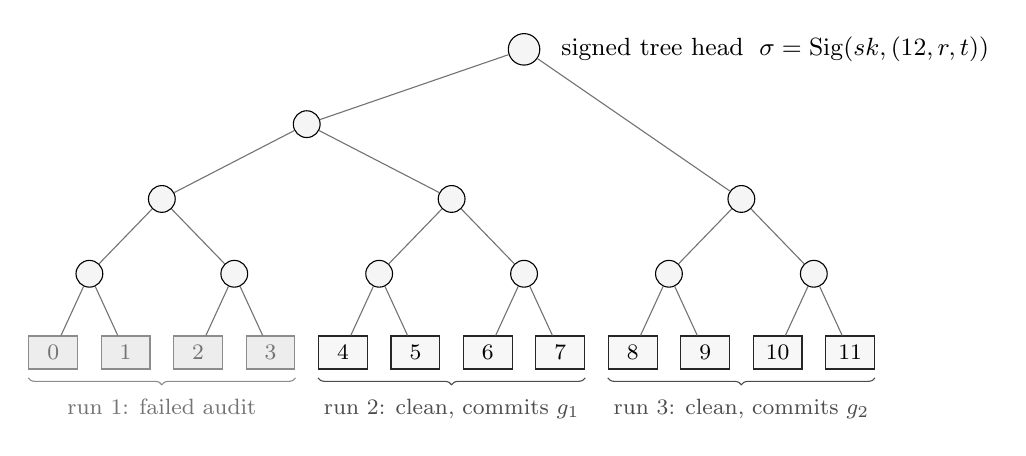
\begin{tikzpicture}[
  every node/.style={font=\footnotesize},
  leaf/.style={draw, minimum width=0.62cm, minimum height=0.42cm, inner sep=1pt},
  fail/.style={leaf, draw=black!45, text=black!55, fill=black!7},
  ok/.style={leaf, draw=black!85, fill=black!3},
  node/.style={draw, circle, minimum size=0.34cm, inner sep=0pt, fill=black!4},
  edge/.style={draw=black!55}, xscale=0.92]
  % leaves 0..11
  \foreach \i in {0,...,3} \node[fail] (l\i) at (\i,0) {\i};
  \foreach \i in {4,...,11} \node[ok] (l\i) at (\i,0) {\i};
  % exact RFC 9162 shape for n = 12: root splits 8 | 4
  \foreach \i/\a/\b in {0/0/1, 1/2/3, 2/4/5, 3/6/7, 4/8/9, 5/10/11}
    \node[node] (m\i) at ({(\a+\b)/2},1.0) {};
  \node[node] (q0) at (1.5,1.95) {};   % leaves 0-3
  \node[node] (q1) at (5.5,1.95) {};   % leaves 4-7
  \node[node] (q2) at (9.5,1.95) {};   % leaves 8-11
  \node[node] (o0) at (3.5,2.9)  {};   % leaves 0-7
  \node[node, minimum size=0.4cm] (root) at (6.5,3.85) {};
  \node[right=1pt of root, font=\small] {\ signed tree head $\;\sigma = \mathrm{Sig}(sk,(12,r,t))$};
  % edges
  \foreach \i/\a/\b in {0/0/1, 1/2/3, 2/4/5, 3/6/7, 4/8/9, 5/10/11}
    { \draw[edge] (l\a)--(m\i); \draw[edge] (l\b)--(m\i); }
  \draw[edge] (m0)--(q0); \draw[edge] (m1)--(q0);
  \draw[edge] (m2)--(q1); \draw[edge] (m3)--(q1);
  \draw[edge] (m4)--(q2); \draw[edge] (m5)--(q2);
  \draw[edge] (q0)--(o0); \draw[edge] (q1)--(o0);
  \draw[edge] (o0)--(root); \draw[edge] (q2)--(root);
  % brackets under leaf ranges
  \draw[decorate,decoration={brace,mirror,raise=3pt}, black!45]
    (l0.south west) -- (l3.south east)
    node[midway,below=7pt, black!55]{run 1: failed audit};
  \draw[decorate,decoration={brace,mirror,raise=3pt}, black!70]
    (l4.south west) -- (l7.south east)
    node[midway,below=7pt]{run 2: clean, commits $g_1$};
  \draw[decorate,decoration={brace,mirror,raise=3pt}, black!70]
    (l8.south west) -- (l11.south east)
    node[midway,below=7pt]{run 3: clean, commits $g_2$};
\end{tikzpicture}
\caption{The deployed twelve-leaf log. Grey leaves 0--3 record the first
run's audit failure (retained, not erased); leaves 4--7 and 8--11 are two
clean runs, at commit generations $g_1$ and $g_2$ across a subject-history
rewrite. The interior is the exact RFC~9162 shape of \S\ref{sec:tree} for
$n = 12$ (root split $8 \mid 4$; $r$ denotes the root value). Every value
in the figure is recomputable from the public leaves.}
\label{fig:tree}
\end{figure}

\begin{table}[t]
\centering\small
\begin{tabular}{@{}lrrl@{}}
\toprule
fork & Lean files & apex cone (axioms, total) & SHA-512 in the boundary \\
\midrule
upstream \texttt{dalek} & 64 & 11 & 3-call streaming (\texttt{new/update/finalize}) \\
Solana (\texttt{anza})  & 58 & \phantom{0}7 & one \texttt{ed\_sigs.sha512\_hash3} \\
RISC~Zero               & 63 & \phantom{0}8 & one \texttt{verifying.sha512\_hash3} \\
Betrusted               & 63 & \phantom{0}8 & one \texttt{verifying.sha512\_hash3} \\
\bottomrule
\end{tabular}
\caption{The four subject implementations. Each replay re-checks 16
certificates in ${\approx}1{,}800$\,s under memory caps and core pinning.
The apex-cone count is the full allowed axiom set at the signature
tiers---Lean's three standard axioms plus the fork's enumerated oracle
boundary (Appendix~\ref{app:axioms}); it differs by fork because the
SHA-512 surface and the byte-accessor shape differ. Proof-script
divergence across forks is quantified in the portability paragraph below;
the pure-mathematics files are byte-identical across all four.}
\label{tab:forks}
\end{table}

\paragraph{What a verified receipt establishes.} Under the assumptions
enumerated below, a consumer who verifies a receipt knows: \emph{the
operator whose key I pinned attests that the Lean certificates of repository
$X$ at commit $Y$ re-check, with per-certificate observed axiom cones as
included---and this statement is part of the log presented to every other
consumer.} Combined with local verdict re-derivation
(Proposition~\ref{prop:verdict}), this yields source-level assurance for the
pinned commit. It deliberately does \emph{not} establish: correctness of any
binary (consumers build from the pinned source; compilers are trusted base),
correctness of SHA-512 (an opaque oracle in the theorems), correctness of
the wire-format parsers (their outcomes are hypotheses of the signature
tiers), signing-side correctness, or side-channel properties.

\paragraph{The assumption set, in full.} The Lean kernel and its three
axioms plus mathlib; faithfulness of the Charon/Aeneas
extraction~\cite{aeneas}; each fork's documented oracle boundary; operator
key custody and trust-on-first-use key distribution (mitigated by publishing
the key in two independent locations); collision resistance of SHA-256 for
the log (Theorems~\ref{thm:sound}, \ref{thm:consistency}); unforgeability
of Ed25519 for the heads (Proposition~\ref{prop:pin}); and the consumer's
own ${\approx}25$-line verifier (Appendix~\ref{app:verifier}).

\paragraph{An observational by-product: proof portability.} Because the
four corpora prove the same theorems against four independent extractions,
the diff between proof files measures how portable proofs are across real
forks. Pure-mathematics files (e.g., a carry-telescope lemma file) are
byte-identical across all four; extraction-facing proof scripts diverge
sharply where the forks' code or the extractor's naming differs (e.g., 215
changed lines for the byte-parser proofs on the two forks whose extraction
produces a closure-based loader; 121 lines for the signature-glue proofs on
the same-crate fork; 27 lines between the two structurally closest forks,
tracking one fork's \texttt{black\_box} optimization barrier and the
operation reordering it induces). Per-target
verification, in other words, is doing
measurable work exactly where the targets actually differ.

\section{Limitations}\label{sec:limitations}

The deployment is small (one operator, twelve leaves, four subject
repositories) and the operator is a single party; split-view defense
currently rests on consumer-side pinning (Proposition~\ref{prop:pin}) plus
the public git mirror rather than an independent witness network. Key
distribution is trust-on-first-use. The signing path of the dogfood binary
is unverified (declared, not proven). The residual trust of
\S\ref{sec:model:residual}---honesty of the operator's kernel
observations---is mitigated only by targeted independent replay, and
replayability presupposes retrievability: a leaf whose pinned commit is
no longer distributed (leaves 0--7 after the subject-history rewrite,
\S\ref{sec:deployment}) decays from a replayable claim to a historical
record, and consumers act on the newest, retrievable attestations. The corpus
itself stops at source-level assurance: reproducible builds and side-channel
evidence remain open, and ML-DSA slots in the head format are deliberately
recorded as unavailable rather than backed by an unverified implementation.

\section{Next step: verifying the accumulator itself}\label{sec:next}

The natural continuation applies the corpus's own discipline to the log's
cryptographic half. Theorems~\ref{thm:complete}--\ref{thm:consistency} and
Proposition~\ref{prop:pin} were stated so as to make their mechanization
direct; we expect the principal work to be specification alignment and
proof engineering rather than new cryptographic argument: (i) inclusion completeness
(Theorem~\ref{thm:complete}) is assumption-free; (ii) inclusion soundness
becomes the explicit extractor of Theorem~\ref{thm:sound}, with SHA-256
collision resistance a documented boundary axiom audited exactly like the
SHA-512 oracle in the Ed25519 tiers; (iii) likewise consistency
(Theorem~\ref{thm:consistency}); (iv) domain separation
(Lemma~\ref{lem:domsep}) is a one-line lemma; and (v) total correctness of
the consumer's pin-store state machine (Proposition~\ref{prop:pin}).
Verified Merkle implementations in F*~\cite{evercrypt} and machine-checked
transparency-protocol analyses~\cite{cheval} show these proofs are well
within reach; the LTL-specific closure is where the certificates go:
\emph{into the log they defend, checked by the certified checker they
specify}, alongside a consumer policy flag requiring the certified verifier.
At that point both proving traditions in the composition run on certified
code, and the remaining trusted base is two hash assumptions, a compiler, an
extraction pipeline, and one key.

\section*{Acknowledgments}

The author designed the system, directed the verification effort, and is
solely accountable for every claim in this paper. Claude (Anthropic) was
used as an assistant in developing the proof corpora, tooling, and text,
and adversarial reviews by both Claude and GPT (OpenAI) shaped the final
manuscript; all
proofs, measurements, and claims have been reviewed by the author and are
independently re-checkable from the public artifacts and the referenced
check scripts.
% \authortodo{The sentence above must be true before you submit it.
% Review every proof in Section 6 line by line and re-run every number in
% Section 8 yourself.}

\begin{thebibliography}{20}
\itemsep2pt

\bibitem{ct1} B. Laurie, A. Langley, E. K\"asper. Certificate Transparency.
RFC 6962, 2013.

\bibitem{ct2} B. Laurie, E. Messeri, R. Stradling. Certificate Transparency
Version 2.0. RFC 9162, 2021.

\bibitem{crosby} S. A. Crosby, D. S. Wallach. Efficient Data Structures for
Tamper-Evident Logging. USENIX Security, pp. 317--334, 2009.

\bibitem{dghs} B. Dowling, F. G\"unther, U. Herath, D. Stebila. Secure
Logging Schemes and Certificate Transparency. ESORICS, LNCS 9879, pp.
140--158, 2016.

\bibitem{sigstore} Z. Newman, J. S. Meyers, S. Torres-Arias. Sigstore:
Software Signing for Everybody. ACM CCS, pp. 2353--2367, 2022.

\bibitem{intoto} S. Torres-Arias, H. Afzali, T. K. Kuppusamy, R. Curtmola,
J. Cappos. in-toto: Providing farm-to-table guarantees for bits and bytes.
USENIX Security, pp. 1393--1410, 2019.

\bibitem{coniks} M. S. Melara, A. Blankstein, J. Bonneau, E. W. Felten,
M. J. Freedman. CONIKS: Bringing Key Transparency to End Users. USENIX
Security, pp. 383--398, 2015.

\bibitem{pcc} G. C. Necula. Proof-Carrying Code. ACM POPL, pp. 106--119,
1997.

\bibitem{cheval} V. Cheval, J. Moreira, M. Ryan. Automatic verification of
transparency protocols. IEEE EuroS\&P, pp. 107--121, 2023.
doi:10.1109/EuroSP57164.2023.00016. arXiv:2303.04500.

\bibitem{easycrypt} G. Barthe, B. Gr\'egoire, S. Heraud, S. Zanella
B\'eguelin. Computer-Aided Security Proofs for the Working Cryptographer.
CRYPTO, LNCS 6841, pp. 71--90, 2011.

\bibitem{aeneas} S. Ho, J. Protzenko. Aeneas: Rust verification by
functional translation. Proc. ACM Program. Lang. 6 (ICFP): 711--741, 2022.

\bibitem{lean4} L. de Moura, S. Ullrich. The Lean 4 Theorem Prover and
Programming Language. CADE-28, LNCS 12699, pp. 625--635, 2021.

\bibitem{hacl} J.-K. Zinzindohou\'e, K. Bhargavan, J. Protzenko,
B. Beurdouche. HACL*: A Verified Modern Cryptographic Library. ACM CCS,
pp. 1789--1806, 2017.

\bibitem{evercrypt} J. Protzenko et al. EverCrypt: A Fast, Verified,
Cross-Platform Cryptographic Provider. IEEE S\&P, pp. 983--1002, 2020.

\bibitem{fiatcrypto} A. Erbsen, J. Philipoom, J. Gross, R. Sloan,
A. Chlipala. Simple High-Level Code for Cryptographic Arithmetic---With
Proofs, Without Compromises. IEEE S\&P, pp. 1202--1219, 2019.

\bibitem{eddsa} D. J. Bernstein, N. Duif, T. Lange, P. Schwabe, B.-Y. Yang.
High-speed high-security signatures. J. Cryptographic Engineering 2(2):
77--89, 2012.

\bibitem{rfc8032} S. Josefsson, I. Liusvaara. Edwards-Curve Digital
Signature Algorithm (EdDSA). RFC 8032, 2017.

\bibitem{edwards} D. J. Bernstein, T. Lange. Faster addition and doubling on
elliptic curves. ASIACRYPT, LNCS 4833, pp. 29--50, 2007.

\bibitem{twisted} D. J. Bernstein, P. Birkner, M. Joye, T. Lange,
C. Peters. Twisted Edwards curves. AFRICACRYPT, LNCS 5023, pp. 389--405,
2008.

\bibitem{pnueli} A. Pnueli. The temporal logic of programs. IEEE FOCS, pp.
46--57, 1977.

\end{thebibliography}

\appendix

\section{Leaf schema}\label{app:leaf}

Each leaf is the canonical JSON serialization (sorted keys, no
insignificant whitespace, UTF-8) of an attestation. Below is leaf~8 of
the deployed log---the re-attestation of the upstream fork. The
16-certificate array is elided to its first (foundational) and last
(apex) entries; long values (hashes, timestamps, version strings,
paths) are shortened, and omitted fields are marked, with ellipses; and
fields are shown in logical rather than canonical (sorted-key) order
for readability. The
field names and values shown, and the axiom lists, are verbatim, and the
unelided leaf is one \texttt{jq} invocation away in the public mirror.
\begin{quote}\ttfamily\scriptsize
\{ "type": "pacta.attestation", "schema\_version": 1,\\
\hspace*{0.6em}"attestation": \{\\
\hspace*{1.2em}"provider": "local-pacta-provider",\\
\hspace*{1.2em}"issued\_at": "2026-07-07T...Z",\\
\hspace*{1.2em}"subject": \{ "component": "dalek-ed25519-verified",\\
\hspace*{2.4em}"repo\_commit": "33fb8bb2311c70ead2e83c0...",\\
\hspace*{2.4em}"repo\_url": ..., "verified\_backend": "serial/u64",\\
\hspace*{2.4em}... \},\\
\hspace*{1.2em}"environment": \{\\
\hspace*{2.4em}"lean\_version": "Lean (version 4.30.0-rc2, ...)",\\
\hspace*{2.4em}"lake\_version": ..., "env\_script": ...,\\
\hspace*{2.4em}"lean\_project\_dir": ... \},\\
\hspace*{1.2em}"machine\_protection": \{ "lean\_guard": ...,\\
\hspace*{2.4em}"note": "All Lean compiles route through the\\
\hspace*{2.4em}repo's lean-guard (memory cap, core pinning,\\
\hspace*{2.4em}timeout, single-flight lock) ..." \},\\
\hspace*{1.2em}"replay": \{ "checked\_files": 64, "failed\_files": [],\\
\hspace*{2.4em}"check\_ok": true, "axiom\_ok": true, ... \},\\
\hspace*{1.2em}"certificates": [\\
\hspace*{2.4em}\{ "name": "CurveFieldProofs.fieldImplementation",\\
\hspace*{3.0em}"status": "proven", "axiom\_status": "clean",\\
\hspace*{3.0em}"observed\_axioms": ["propext",\\
\hspace*{3.6em}"Classical.choice","Quot.sound"],\\
\hspace*{3.0em}"expected\_axioms": [...], ... \},\\
\hspace*{2.4em}... \; \emph{(14 certificates elided)} \; ...\\
\hspace*{2.4em}\{ "name":\\
\hspace*{3.0em}"CurveFieldProofs.verify\_accepts\_iff\_decompress",\\
\hspace*{3.0em}"status": "proven", "axiom\_status": "clean",\\
\hspace*{3.0em}"observed\_axioms": ["propext","Classical.choice",\\
\hspace*{3.6em}"Quot.sound","ed25519.Signature","sha2.Sha512",\\
\hspace*{3.6em}"verifying.sha512\_finalize\_bytes",\\
\hspace*{3.6em}"verifying.sha512\_new","verifying.sha512\_update",\\
\hspace*{3.6em}"ed25519.Signature.to\_bytes",\\
\hspace*{3.6em}"signature.error.Error",\\
\hspace*{3.6em}"signature.error.Error.new"], ... \} ],\\
\hspace*{1.2em}"signature": \{ "scheme": "openssl-ed25519", ... \},\\
\hspace*{1.2em}... \} \}
\end{quote}
The \texttt{observed\_axioms} field is the exact output of
\texttt{\#print axioms} for that theorem. Operator labels
(\texttt{replay.check\_ok}, per-certificate \texttt{status} and
\texttt{axiom\_status}) are recorded for the audit trail, but the
cleanliness verdict is $\obs = \allowed$ computed against the consumer's
own table in every case, with a missing cone mapped to
\textsf{unverifiable} (Proposition~\ref{prop:verdict}). The
\texttt{status} label is consulted only \emph{negatively}: a certificate
the operator itself does not mark proven can never count toward
acceptance, so labels can deny but never grant.

\section{The consumer verifier}\label{app:verifier}

The consumer-side inclusion check, in full (Python, standard library only);
this is the recursive form proved in \S\ref{sec:security} and is equivalent
to the iterative algorithm of RFC~9162 \S2.1.3.2.

\begin{quote}\ttfamily\small
import hashlib\\[2pt]
def H(b): return hashlib.sha256(b).digest()\\
def h\_leaf(d): return H(b'\textbackslash x00' + d)\\
def h\_node(x, y): return H(b'\textbackslash x01' + x + y)\\[2pt]
def largest\_pow2\_below(n):\\
\hspace*{1em}k = 1\\
\hspace*{1em}while 2 * k < n: k *= 2\\
\hspace*{1em}return k\\[2pt]
def root(v, m, n, path):\\
\hspace*{1em}if n == 1:\\
\hspace*{2em}if path: raise ValueError\\
\hspace*{2em}return v\\
\hspace*{1em}if not path: raise ValueError\\
\hspace*{1em}*rest, s = path\\
\hspace*{1em}k = largest\_pow2\_below(n)\\
\hspace*{1em}if m < k:\\
\hspace*{2em}return h\_node(root(v, m, k, rest), s)\\
\hspace*{1em}return h\_node(s, root(v, m - k, n - k, rest))\\[2pt]
def verify\_inclusion(leaf, m, n, path, head\_root):\\
\hspace*{1em}return m < n and root(h\_leaf(leaf), m, n, path) == head\_root
\end{quote}
Signature verification of the head (Ed25519) and the pin-store logic of
\S\ref{sec:pinstore} complete the consumer; the deployed
${\approx}150$-line standalone verifier in the mirror additionally checks
consistency proofs and recomputes prefix roots from the public leaves.

\section{Allowed axiom sets}\label{app:axioms}

Foundational certificates (12 of 16) must carry exactly Lean's three
standard axioms:
\begin{quote}\ttfamily\small
propext \quad Classical.choice \quad Quot.sound
\end{quote}
The four signature-tier certificates additionally carry a per-fork
enumerated boundary: an opaque SHA-512 oracle and opaque wire-format
types (the signature type, its byte accessors, and---where the fork's
API surfaces it---the error type). The
boundary is not identical across forks---it reflects each fork's actual
extracted surface---and auditing is exact against the fork's own set. The
three distinct boundaries in the deployed corpus, verbatim from the
repositories' check scripts, are as follows (the three standard axioms
above, plus):

\smallskip
\noindent\textbf{Upstream \texttt{curve25519-dalek}} (11 axioms total;
this fork exposes SHA-512 as three streaming operations):
\begin{quote}\ttfamily\scriptsize
ed25519.Signature \quad sha2.Sha512\\
verifying.sha512\_finalize\_bytes\\
verifying.sha512\_new \quad verifying.sha512\_update\\
ed25519.Signature.to\_bytes\\
signature.error.Error \quad signature.error.Error.new
\end{quote}

\noindent\textbf{RISC~Zero and Betrusted forks} (8 axioms total;
identical to each other---SHA-512 is a single \texttt{hash3} oracle):
\begin{quote}\ttfamily\scriptsize
ed25519.Signature \quad verifying.sha512\_hash3\\
ed25519.Signature.to\_bytes\\
signature.error.Error \quad signature.error.Error.new
\end{quote}

\noindent\textbf{Solana (anza) fork} (7 axioms total; its own
\texttt{ed\_sigs} namespace, and \texttt{R}/\texttt{s} byte accessors
rather than a whole-signature encoder):
\begin{quote}\ttfamily\scriptsize
ed25519.Signature \quad ed\_sigs.sha512\_hash3\\
ed25519.Signature.r\_bytes \quad ed25519.Signature.s\_bytes
\end{quote}

A consumer's local table (\S\ref{sec:auditing}) contains exactly these
sets. That a boundary differs by fork is itself audited: an
upstream-shaped cone appearing under the anza label, or vice versa, fails
$\clean$ in the ``unexpected axiom'' direction.

\section{The four verification tiers: Lean theorem names}\label{app:tiers}

The lifting ladder T1--T4 and the mathematical facts it turns on are
stated in \S\ref{sec:corpus}. For reproducibility we record here the
verbatim Lean theorem name backing each tier in the upstream corpus
(namespace \texttt{CurveFieldProofs} elided; the forks use the same names
against their own extractions); a reader can
\texttt{\#print axioms} any of these to reproduce the cones of
Appendix~\ref{app:axioms}.
\begin{center}\small
\begin{tabular}{@{}ll@{}}
\toprule
tier (\S\ref{sec:corpus}) & Lean theorem \\
\midrule
T1 \enspace byte apex          & \texttt{verify\_accepts\_iff} \\
T2 \enspace canonical half-lift & \texttt{verify\_accepts\_iff\_point} \\
T3 \enspace injectivity / point eq. & \texttt{verify\_accepts\_iff\_point\_eq} \\
T4 \enspace constructive full lift & \texttt{verify\_accepts\_iff\_decompress} \\
\bottomrule
\end{tabular}
\end{center}
All four are proven under the wire-format hypotheses $\mathcal{W}$ of
\S\ref{sec:corpus}; a consumer reasoning about the underlying group
element relies on their conjunction (the ladder up to T4), and all four
cones are audited against the same per-fork boundary of
Appendix~\ref{app:axioms}.

\end{document}
